
%(BEGIN_QUESTION)
% Copyright 2010, Tony R. Kuphaldt, released under the Creative Commons Attribution License (v 1.0)
% This means you may do almost anything with this work of mine, so long as you give me proper credit

A PLC is used to sequence the operation of a {\it lock hopper} used to feed pulverized coal into a gasification reactor where the coal is heated to release flammable gases useful as fuels.  Many details on the reactor have been omitted from this diagram for simplicity:

$$\includegraphics[width=15.5cm]{i03732x01.eps}$$

The purpose of the ``lock hopper'' is to prepare a charge of coal for injection into the reactor while maintaining gas pressure in the reactor (i.e. not letting the flammable coal gases escape) and also not letting any air into the reactor where it could support an explosion.

The basic sequence of the lock hopper is as follows: (1) wait for command signal from production control system to inject more coal into gasifier reactor; (2) wait for proof of valve \#2 closure, then open lock valve \#1 to introduce coal into lock hopper vessel; (3) wait for high level switch (LSH) to trip, then close lock valve \#1; (4) wait for proof of valve \#1 closure, then open steam inlet and outlet valves to purge lock-hopper of air for a set time period; (5) close steam outlet valve to allow lock-hopper to pressurize until its pressure is equal to the pressure measured inside the gasifier reactor; (6) open lock valve \#2 for a set time period; (7) close steam inlet valve and close lock valve \#2.

\vskip 10pt

Suppose one day the proof-of-closure switch on lock valve \#2 fails in such a way that it reports the valve as being open all the time even when it is closed tight.  Explain how this switch failure will affect the operation of the lock hopper as controlled by the PLC.

\vskip 10pt

Furthermore, suppose an instrument technician is called to investigate this problem, and decides to fix it by ``forcing'' the input bit of the PLC so that it sees the lock valve \#2 as being closed despite the broken switch's status.  This allows the process to continue running while the technician then repairs the switch.  Explain why this might not be a good way to proceed, and be specific in your answer!

\vfil 

\underbar{file i03732}
\eject
%(END_QUESTION)





%(BEGIN_ANSWER)

This is a graded question -- no answers or hints given!

%(END_ANSWER)





%(BEGIN_NOTES)

Without proof of valve \#2's closure, the PLC sequence will become stuck at step 2.  Since the PLC program is designed to refrain from opening up lock valve \#1 until valve \#2 is proven to be in the ``closed'' position, it will never see that requisite condition to allow any fresh coal to enter the lock hopper.  Thus, the automated coal-feeding sequence will be stalled and the reactor will run out of feed.

\vskip 10pt

Forcing the PLC's input bit to register the valve as being closed will allow the sequence to advance past step 2, but it may also pose a danger because now the system thinks valve \#2 is closed even when it might not actually be closed!  For example, at the next iteration of step 2, if lock valve \#2 happens to not close as it should, lock valve \#1 will open anyway and allow flammable coal gas to escape from the reactor into the coal feed line, where it could cause a fire and/or explosion!

%INDEX% Basics, control loop troubleshooting: determining effect of specified fault(s)
%INDEX% Process: coal gasification (gasifier reactor)

%(END_NOTES)

